\documentclass[a4paper,11pt]{article}
\usepackage[T1]{fontenc}
\usepackage[utf8]{inputenc}
\usepackage{lmodern}

\usepackage{makeidx}
    % Needed to build the index.

\usepackage{amsmath}
    % Brings the align environment for lining up equations on the =.

\usepackage{amssymb}
    % For the number set symbols.

\usepackage{cancel}
    % For striking out bits of equations that simplify.

\usepackage{graphicx}
    % Can't have pictures/photos/figures from files without that.
    % Note that vanilla latex will only accept eps.
    
\usepackage{subfigure}
    % Lets me have labels such as a) b) c) inside a figure environment.

\usepackage[font=footnotesize, labelfont=bf]{caption}
    % So that I can add long captions under figures.
    % It provides me with \caption* that does not appear in the list of
    % figures but formats the text like \caption does.  It also lets me
    % use line breaks in the caption, and even bullet/enumerated lists.

\usepackage{color}
    % For rendering text is eps_tex files produced by InkScape, even
    % if the text is black.

\usepackage{booktabs}
    % For professional-looking tables.
    % Brings the \toprule, \midrule and \bottomrule.
    % Remember not to use vertical rules in tables: they look cheap.

\usepackage[version=3]{mhchem}
    % For chemical formulas.
    % Brings \ce.ormulas.

\usepackage{stmaryrd}
    % For the llbracket and rrbracket to denote integer intervals.

\usepackage{varioref}
    % For fancier references that also tell the page number.
    
\usepackage{todonotes}
    % Big post-its, handy while writing.
    
\usepackage[]{biblatex}
    % Fantastic bibliography manager that I'll use just for its
    % \citetitle command.

%\usepackage[mediumspace,mediumqspace,squaren]{SIunits}
\usepackage{siunitx}
    % Otherwise I can't write the mu symbol for micrometers.
    % It also brings me the \degree symbol, woo!
    % No decibel though, I need to make this one myself.
\newcommand{\decibel}{dB}
\newcommand{\equaldef}{\stackrel{\text{\tiny def}}{=}}
\newcommand{\transp}{^T}
\newcommand{\norm}[1]{\left\| #1 \right\|}
\newcommand{\abs}[1]{\left| #1 \right|}

\graphicspath{{./figures/}}
\addbibresource{bibliography.bib}

\title{Understanding standing waves by network modeling
\\
\large{HIFI untangled, and prospects for future instrumentation}}
\author{Bertrand Delforge$^{1, 2}$
       \and
       John Pearson$^3$
       \and
       Peter Roelfsema$^{1, 2}$
       \and
       Marc Verheijen$^2$
       \and
       Willem Jellema$^1$
       \and
       \\ \footnotesize $^1$ SRON, Netherlands Institute for Space Research
       \\ \footnotesize $^2$ Kapteyn Astronomical Institute
       \\ \footnotesize $^3$ JPL, Jet Propulsion Laboratory
}

\begin{document}

\maketitle
%\tableofcontents

\begin{abstract}
As is the case for many coherent instruments like HIFI, the Heterodyne Instrument for the Far Infrared on the Herschel space observatory, standing waves affect the nominal coupling of the mixer to the local oscillator, calibration black bodies and even the sky.  This results in obvious distortions of the spectral baselines and strongly influences other parameters such as the sideband ratio.  Current uncertainties on HIFI's sideband ratio are about 2-10 percent, depending on the frequency, and are mainly a consequence of an insufficient understanding of the HIFI standing wave phenomenon.

We are developing a systematic and generic methodology for modeling standing waves in coherent optical and quasi-optical systems, using scattering matrices combined with Jones matrices.
This approach allows for a consistent processing of both the phase and polarization information of multi-port networks, and serves as a foundation to combine an arbitrarily large number of networks and predict their interactions.

Our numerical simulations successfully reproduce, and qualitatively explain, many artifacts observed in actual HIFI data.
We are currently improving our technique to produce quantitative predictions.
With HIFI as a hands-on show case for our successful standing wave modeling technique,
we are confident that this generic approach for understanding and predicting standing waves can play a significant role in improving the design of future instruments.
\end{abstract}





%=============================================================================

\section{Introduction}
The HIFI instrument on the Herschel Space Observatory \cite{AA_518_L1} is a heterodyne receiver that operates at frequencies between \SI{480}{\giga\hertz} and \SI{1910}{\giga\hertz},
producing spectra with a resolution ranging from \SI{1}{\mega\hertz} to \SI{125}{\kilo\hertz} \cite{AA_518_L6}.
This high frequency resolution enables the astronomers to study the chemistry of a wide range of phenomena, from planetary atmospheres to star forming regions.

At such a high resolution, the thermal noise of the astronomical source, the calibration black bodies and the local oscillator (LO) qualify as ``narrow band Gaussian noise signals'' \cite{siegman1986lasers}.
They have a coherence time~$\tau$ equal to the inverse of their bandwidth~$\tau=1/\Delta f$.
A bandwith of~\SI{1}{\mega\hertz} results in a coherence time of \SI{1}{\micro\second} equivalent to a coherence length of \SI{300}{\meter}.
This is a hundred times the longest distance inside HIFI.
Therefore, in HIFI, the signals from the LO, the calibration sources and the sky are coherent.

In a coherent system, interferences can appear.
Interference inside electromagnetic cavities give rise to standing waves which trap energy inside these cavity.
The energy that is trapped inside a cavity is not available for frequency conversion by the mixer.
In other words, the mixer coupling of the incoming signals is modulated by these standing waves.

\begin{figure}[hbt]
    \centering
    % CO 9-8 line of NCG7538-IRS1 observed on 21-02-2010.
    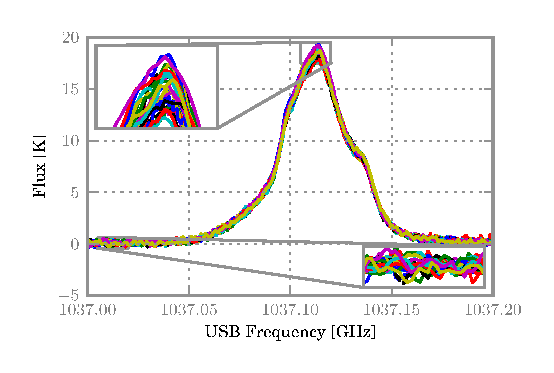
\includegraphics{obsid_5000352C}
    \caption{\label{fig:scatter_real_data}
    The left plot shows the same extragalactic emission feature observed by HIFI at 25 different LO frequencies in its band 4a.
    The scatter on the line peak is greater than the expected noise (inset plots).
    The peak fluxes and the corresponding noise levels are reported in the right plot: the error bars representing the noise.
    The scatter on the peak flux is three times greater than the noise.
    }
\end{figure}

Figure~\ref{fig:scatter_real_data} illustrates this phenomenon for a very subtle case
(the calibration paper~\cite{AA_537_A17} illustrates more obvious ones).
HIFI observed a single emission feature from a galactic source for 25 local oscillator frequencies.
If there were no standing waves, or if the standing waves were perfectly calibrated out, then all these line profiles would overlap within the noise.
Instead, their peak intensity is scattered by more than the expected noise.
This scatter is due to standing waves that are ignored by the calibration: each LO frequency requires a specific tuning of the diplexer, which changes the optical paths, which changes the periods of the standing waves, which changes the mixer coupling to the sky, LO and calibration loads.
This case is a subtle one: each of these 25 spectra looks individually clean from standing wave modulations (no apparent periodic distortion of the spectrum), only their comparison reveals the effect of standing waves.
Standing waves introduce a systematic uncertainty that cannot be reduced by integrating longer.
When an observation is taken at one LO frequency only, the astronomer has little to no way of knowing how much standing waves distort the line.

Our goal is to model the instrument to a level which allows to accurately predict the effect of the standing waves, and include a correction of their effect in the calibration scheme of HIFI.





%=============================================================================

\section{Modeling standing waves}



%-----------------------------------------------------------------------------

\subsection{Principle}
Our method is inspired from laser and circuit theory: we deal with discrete inputs and outputs rather than, for example, a spatial description of the fields.
A system like the Focal Plane Unit of HIFI comprises a few dozens of optical elements, refered in the litterature as ``networks'' \cite{siegman1986lasers}: wire grid polarizers, roof-top mirrors, horns, attenuators, free space, all having one or more input and output.
All these networks interact together two by two since there exists at least one optical path between each pair or networks.
The number of interactions in the system increases with the square of the number of networks.
One way to solve a system's reaction to a set of input would be to propagate the inputs from network to network, back and forth, until the fields appear to converge to a steady state.
Instead, we propose a method to reduce the number of networks without losing any information, in a way that can be compared to calculating the equivalent impedance of an electric circuit.
Our model computes the scattering matrix of the network equivalent to the whole system.
Then, knowing how the system reacts to an input is merely a matter of multiplying its scattering matrix with a vector of inputs to get a vector of outputs.

Scattering matrices \cite{siegman1986lasers} model the transfer of power or field from one side (port) of a network to another (figure~\ref{fig:ports}).
\begin{figure}[hbtp]
    \centering
    \input{figures/scattering_matrix_notations.eps_tex}
    \caption{\label{fig:ports}A 4-ports network showing 4 inputs $a_i$ and four outputs $b_i$.  For example, this network could be a wire grid polarizer or a semi-transparent mirror, both acting as beam splitters.}
\end{figure}
Equation~\ref{eq:scattering_matrix} presents the scattering matrix $S$ that models the relation between a vector of inputs $a$ and a vector of outputs $b$ for a $n$-ports network.
The diagonal contains the reflections terms and the rest contains the transmissions.
\begin{align}
    b &= S a
    &
    \begin{pmatrix}
        b_1\\
        b_2\\
        \vdots\\
        b_n
    \end{pmatrix}
    &=
    \begin{pmatrix}
        S_{1, 1} & S_{1, 2} & \cdots & S_{1, n} \\
        S_{2, 1} & S_{2, 2} & \cdots & S_{2, n} \\
        \vdots   & \vdots   & \ddots & \vdots   \\
        S_{n, 1} & S_{n, 2} & \cdots & S_{n, n}
    \end{pmatrix}
    \begin{pmatrix}
        a_1\\
        a_2\\
        \vdots\\
        a_n
    \end{pmatrix}
    \label{eq:scattering_matrix}
\end{align}
The standard way to include the polarization into a scattering matrix is to double (local reference frame: horizontal and vertical directions) or triple (global reference frame: $x$, $y$ and $z$ directions) its number of ports.
For our model, we chose a different approach that allows us consider a polarized field as a single entity instead of two or three, and keep the number of ports to a minimum.
For this, we adapt the traditional scattering matrix formalism to our need:
the elements~$S_{i, j}$ of the scattering matrix~$S$ are not scalars, but Jones matrices.

Jones matrices model the transfer of amplitude and phase from one polarization to another \cite{hecht2002optics}.
In equation~\eqref{eq:jones_matrix_short}, the polarized input field $e_i$ is related to the polarized output field~$e_o$ by the Jones matrix $J$.
$e_i$ and $e_o$ are called ``Jones vectors''.
\begin{equation}
    % Small form.
    e_o = J e_i
    \label{eq:jones_matrix_short}
\end{equation}
The components of the Jones vectors are phasors: complex numbers that encode the amplitude and phase of the field along different axes.
The components of the Jones matrices are also complex numbers, these encode changes in amplitude and phase.

Equation~\eqref{eq:jones_matrix_2d} presents the traditional form of Jones vectors and matrices.
\begin{equation}
    % Jones matrix in 2D.
    \begin{pmatrix}
        e_{o, h}\\
        e_{o, v}
    \end{pmatrix}
    =
    \begin{pmatrix}
        J_{h, h}   &   J_{h, v} \\
        J_{v, h}   &   J_{v, v}
    \end{pmatrix}
    \begin{pmatrix}
        e_{i, h}\\
        e_{i, v}
    \end{pmatrix}
    \label{eq:jones_matrix_2d}
\end{equation}
The field is seen as the superposition of a horizontal and a vertical component, both linearly polarized.
The phase difference between these components determines the handedness and the ellipticity of the polarization of the field.
Although very useful for many applications, these Jones matrices and vectors have limitations.

First, the field is always expressed in a local reference frame: the horizontal and vertical directions are valid for one beam only and may change after any reflection or refraction.
Therefore, to completely describe a field, the Jones vector is not enough since one needs to keep track of the orientation of its reference frame with three angles, a quaternion or a rotation matrix.

Second, the horizontal and vertical directions are normal to each other and to the direction of propagation.
This limits us to modeling either TE or TM waves\footnote{transverse electric, transverse magnetic} depending on whether the Jones vector represents the electric or the magnetic field.
However, this cannot model hybrid waves, in which both the electric and the magnetic field can have a component along the direction of propagation.
Therefore, this cannot model propagation in a birefringent material.
One way to accomodate this is to relax the constraint of orthogonality of the reference frame, allowing for the horizontal and vertical directions to have a component along the direction of propagation.
If we do this, then the full description of the field gets even more complicated as we need to carry along, not just the orientation of its reference frame, but the full description of that non-cartesian reference frame.

Instead, we can express all the fields in a common global cartesian reference frame, essentially extending Jones calculus from two to three dimensions, as illustrated in equation~\eqref{eq:jones_matrix_3d}.
\begin{equation}
    % Jones matrix in 3D.
    \begin{pmatrix}
        e_{o, x}\\
        e_{o, y}\\
        e_{o, z}
    \end{pmatrix}
    =
    \begin{pmatrix}
        J_{x, x}   &   J_{x, y}   &   J_{x, z} \\
        J_{y, x}   &   J_{y, y}   &   J_{y, z} \\
        J_{z, x}   &   J_{z, y}   &   J_{z, z}
    \end{pmatrix}
    \begin{pmatrix}
        e_{i, x}\\
        e_{i, y}\\
        e_{i, z}
    \end{pmatrix}
    \label{eq:jones_matrix_3d}
\end{equation}

\begin{figure}[hbtp]
    \centering
    \input{figures/cascading.eps_tex}
    \caption{\label{fig:cascading}Two networks P~and~Q connected by one port are equivalent to a network S.}
\end{figure}
As shown on figure~\ref{fig:cascading}, two networks~P and~Q connected by one port can be seen as a single equivalent network~S.
Our model can compute the scattering matrix of~S from the scattering matrices of~P and~Q for any P~and~Q connected by any port.
The scattering matrix of S takes into account the infinite reflections on the ports by which P~and~Q are connected.

Once we have this method to compute~S from~P and~Q, then we apply it recursively to get the scattering matrix of the whole system.
This is illustrated by figure~\ref{fig:cascading_example}, where we use a HIFI diplexer unit as an example and reduce it to a single network.
\begin{figure}[hbtp]
    \centering
    \input{figures/cascading_example.eps_tex}
    \caption{\label{fig:cascading_example}
    A system comprising several networks connected by one port can be reduced to a single equivalent network.
    This is done by recursively combining networks two by two until there is only one network left.
    This example presents a HIFI diplexer unit; it contains two rooftop mirrors (pentagons) and a wire grid polarizer (dotted line) separated by free space (rectangles), its purpose is to align the polarization of the LO and the sky signals in order to couple both to the mixer (crossed circle).
    }
\end{figure}

Our method is recursive but not iterative: it passes over each network only once.
Once the scattering matrix of the whole system is calculated, we have direct access to the steady state of that system.

The detail of the mathematics and algorithms used in this model falls out of the scope of this paper and shall be presented in a later publication~\cite{delforge_2014_phdthesis}.

%-----------------------------------------------------------------------------

\subsection{Simplifications}

HIFI operates in the sub-millimeter regime where the wavelength is of the same order as the dimensions of the networks.
We could use quasi optics to properly account for the diffraction of the beams \cite{goldsmith1998quasioptical}.
However, our model assumes plane, and therefore single-mode, waves.
The plane-wave hypothesis is acceptable at a first order because the networks are placed at the waist of the beams where the wave front is plane.
Furthermore, the discrepancies due to these simplifications can be abstracted by parameters in our model.
For example, if a higher mode does not couple to a mixer, then its power is --for all practical purpose-- lost, and therefore a term of loss can model it.

Our model can be extended to higher order modes.
This can be done by adding components to the Jones vectors/matrices, or by adding an additional layer of matrices between the scattering matrix and the Jones matrix, which would take care of the transfer of power between modes.


\paragraph{Typical networks.}
Most typical networks can be easily modeled at the first order;
we generate their scattering matrices with parameters such as refractive index, thickness, orientation in space, attenuation, etc..
Wire grid polarizers are much more difficult to model; we adapted the work of \citeauthor{houde_2001}~\cite{houde_2001} to out matrix format.



%=============================================================================

\section{Qualitative achievement}

Using the method presented in this article, we modeled the optical part of HIFI, that is the networks 
A typical HIFI observation consists in four integrations: one on the astronomical source, one on a reference position in the sky, and two internal black bodies used for intensity calibration.

In order to reproduce the behavior illustrated in figure~\ref{fig:scatter_real_data}, we present four sources to that model: a perfect Gaussian line of~\SI{18}{\kelvin} on top of a~\SI{1}{\kelvin} continuum, a reference source with no signal (no continuum no line), and on two calibration black bodies at \SI{10}{\kelvin} and \SI{100}{\kelvin}.
Each of these integrations also sees noise from the local oscillator, approximated with a~\SI{120}{\kelvin} black body.
The result is given in figure~\ref{fig:calibrated_std}
\begin{figure}[hbtp]
    \centering
    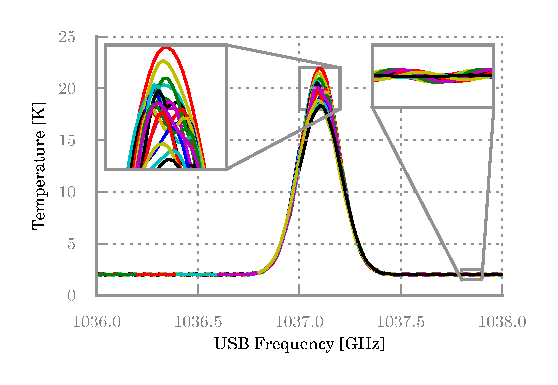
\includegraphics{bb-on_corrected-2}
    \caption{\label{fig:calibrated_std}Simulated line with standard HIFI calibration for 25 LO frequencies.
    Standing waves introduce a weak periodic modulation of the baseline and a strong scatter of the peak intensity of the line.}
\end{figure}
Figure~\ref{fig:calibrated_std} shows that our model properly reproduces the scatter seen on real data (figure~\ref{fig:scatter_real_data}).
It also reveals the effect of standing waves on the baseline, but this effect is drowned in the noise.

\begin{figure}
    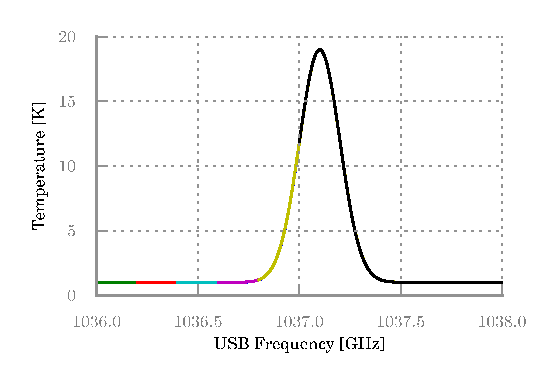
\includegraphics[width=.45\textwidth]{bb-on_corrected-3}
    \caption{\label{fig:calibrated_sbr}Calibration scheme that uses the sideband ratio provided by the model.}
%    \caption{\label{fig:calibrated}Simulated spectra.
%    Each LO tuning brings its own set of standing waves that modulate the couplings to the different sources.
%    Without knowledge of these couplings, the calibration is not perfect.
%    The model gives us some information that allows us to properly calibrate out all the standing waves.}
\end{figure}

Our model gives us information that is absent from real data: the sideband ratio.
Standing waves, being frequency-dependent, modulate the lower and upper sidebands differently, resulting in an imbalanced ratio between the two sidebands during the folding by the mixer, see figure~\ref{fig:sbr}
By using the sideband ratio predicted by the model, we are able to properly calibrate our simulated spectrum, as illustrated in figure~\ref{fig:calibrated_sbr}.
\begin{figure}[hbtp]
    \centering
    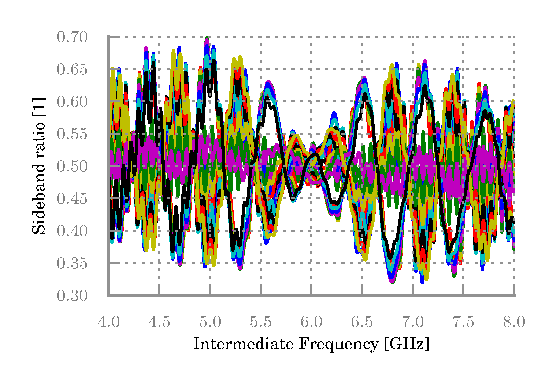
\includegraphics{sbr}
    \caption{\label{fig:sbr}Simulated sideband ratio for a diplexer band of HIFI at 25 different LO~frequencies.
    The sideband ratio is defined in terms of the LSB and USB gains as $G_\text{USB}/(G_\text{LSB} + G_\text{USB})$.  Its ideal value is 0.5; above 0.5, the channel is USB-dominated, and under 0.5 it is LSB-dominated.
    The sideband ratio varies quickly over the IF, as several standing wave patterns beat and modulate each other.
    The \SI{620}{\mega\hertz}-wide periodic modulation comes from the standing wave between the mixers and the closest roof-top mirrors of the diplexer assemblies.  The wide envelop results from the fact that the diplexer tuning is optimal at the center of the IF and degrades on the edges.  We can also see a~\SI{150}{\mega\hertz} pattern that correspond to the LO-mixer cavities.}
\end{figure}





%=============================================================================

\section{Conclusion}
We have designed and implemented a framework to model the interferences, and therefore the standing waves, in any coherent instrument.
The model produces results that are qualitatively consistent with many HIFI observations.
We showed that the model can give us information (notably the sideband ratio) that we can use to better calibrate data.
By modeling more accurately the networks, we are expecting to reproduce quantitatively HIFI data.
This would allow us to significantly reduce the uncertainties in the calibration.

%=============================================================================

\printbibliography
\end{document}
